\documentclass[11pt]{article}\usepackage[]{graphicx}\usepackage[]{color}
%% maxwidth is the original width if it is less than linewidth
%% otherwise use linewidth (to make sure the graphics do not exceed the margin)
\makeatletter
\def\maxwidth{ %
  \ifdim\Gin@nat@width>\linewidth
    \linewidth
  \else
    \Gin@nat@width
  \fi
}
\makeatother

\definecolor{fgcolor}{rgb}{0.345, 0.345, 0.345}
\newcommand{\hlnum}[1]{\textcolor[rgb]{0.686,0.059,0.569}{#1}}%
\newcommand{\hlstr}[1]{\textcolor[rgb]{0.192,0.494,0.8}{#1}}%
\newcommand{\hlcom}[1]{\textcolor[rgb]{0.678,0.584,0.686}{\textit{#1}}}%
\newcommand{\hlopt}[1]{\textcolor[rgb]{0,0,0}{#1}}%
\newcommand{\hlstd}[1]{\textcolor[rgb]{0.345,0.345,0.345}{#1}}%
\newcommand{\hlkwa}[1]{\textcolor[rgb]{0.161,0.373,0.58}{\textbf{#1}}}%
\newcommand{\hlkwb}[1]{\textcolor[rgb]{0.69,0.353,0.396}{#1}}%
\newcommand{\hlkwc}[1]{\textcolor[rgb]{0.333,0.667,0.333}{#1}}%
\newcommand{\hlkwd}[1]{\textcolor[rgb]{0.737,0.353,0.396}{\textbf{#1}}}%

\usepackage{framed}
\makeatletter
\newenvironment{kframe}{%
 \def\at@end@of@kframe{}%
 \ifinner\ifhmode%
  \def\at@end@of@kframe{\end{minipage}}%
  \begin{minipage}{\columnwidth}%
 \fi\fi%
 \def\FrameCommand##1{\hskip\@totalleftmargin \hskip-\fboxsep
 \colorbox{shadecolor}{##1}\hskip-\fboxsep
     % There is no \\@totalrightmargin, so:
     \hskip-\linewidth \hskip-\@totalleftmargin \hskip\columnwidth}%
 \MakeFramed {\advance\hsize-\width
   \@totalleftmargin\z@ \linewidth\hsize
   \@setminipage}}%
 {\par\unskip\endMakeFramed%
 \at@end@of@kframe}
\makeatother

\definecolor{shadecolor}{rgb}{.97, .97, .97}
\definecolor{messagecolor}{rgb}{0, 0, 0}
\definecolor{warningcolor}{rgb}{1, 0, 1}
\definecolor{errorcolor}{rgb}{1, 0, 0}
\newenvironment{knitrout}{}{} % an empty environment to be redefined in TeX

\usepackage{alltt}
\usepackage[margin=0.75in]{geometry}            % See geometry.pdf to learn the layout options. There are lots.
\geometry{letterpaper}                                  % ... or a4paper or a5paper or ... 
%\geometry{landscape}                           % Activate for rotated page geometry
%\usepackage[parfill]{parskip}                  % Activate to begin paragraphs with an empty line rather than an indent
\usepackage{graphicx}                           % Use pdf, png, jpg, or eps§ with pdflatex; use eps in DVI mode
                                                                % TeX will automatically convert eps --> pdf in pdflatex                
\usepackage{amssymb}
\usepackage{upquote}
\usepackage{caption}

%-----------------------------------------------------------------------------
% Special-purpose color definitions (dark enough to print OK in black and white)
\usepackage{color}
% A few colors to replace the defaults for certain link types
\definecolor{orange}{cmyk}{0,0.4,0.8,0.2}
\definecolor{darkorange}{rgb}{.71,0.21,0.01}
\definecolor{darkgreen}{rgb}{.12,.54,.11}
%-----------------------------------------------------------------------------
% The hyperref package gives us a pdf with properly built
% internal navigation ('pdf bookmarks' for the table of contents,
% internal cross-reference links, web links for URLs, etc.)
\usepackage{hyperref}
\hypersetup{pdftex, % needed for pdflatex
  breaklinks=true, % so long urls are correctly broken across lines
  colorlinks=true,
  urlcolor=blue,
  linkcolor=darkorange,
  citecolor=darkgreen,
}


\title{Wireless Sensor Network Project\\
  Stat 222, Spring 2016}

\author{
  Thibault Doutre\\
  \texttt{github: doutib}
}

\setkeys{Gin}{width=0.5\textwidth}
\IfFileExists{upquote.sty}{\usepackage{upquote}}{}
\begin{document}
\maketitle

\abstract{The low impact and low visibility of wireless sensors make them very suitable for environmental monitoring. Researchers for the University of California, Berkeley use those wireless sensors to study California's trees in Redwoods, in order to capture spatial and temporal information (e.g., temperature, humidity). The data has been gathered during the early summer of 2004. This paper proposes to reveal trends in the data set.}


\section{Introduction}
In 2003, graduate students with Todd Dawson, professor of integrative biology at the University of California, Berkeley, experimented a wireless sensor network on trees in the Redwoods \cite{yang2003redwoods} in order to better understand the impact of the Californian micro climate on the trees. In June 2004, other people from Berkeley gathered the sensors and extracted the data which had been monitored for a month. In 2005, they published an article \cite{tolle2005macroscope} which gives some insights about the data.

We dispose of two data sets (e.g. locations and values) which respectively contain information about the location of the sensors and the measured values of the sensors over the period of sampling.
The locations data set provides the following information for each node: ID, Height, Orientation, Distance from trunk and whether it has been placed on an edge or in the interior of the tree.
The values data set reports the measurement of the predefined metrics for different times, during the study. In particular, the following values are gathered: The time the measurement was taken, the ID of each measurement time, the ID of the node, the ID of the parent of the node, the voltage, the depth of the node, the humidity, the temperature, the adjusted humidity, the incident photo-synthetically active radiation (PAR) and the reflected PAR. 


\section{The Data}


\subsection{Data Collection}

I will mainly focus on the three following variables: Incident PAR, humidity and temperature.

For the humidity, the sensors have been calibrated for values around 20 and 90 \%RH, for temperatures between 5 and 30 Celsius degrees. To have an idea of the temperature in Redwoods, the range of temperature encountered in the San Francisco in May 2004 is between 7 and 26 Celsius degrees \cite{weatherspark}. This show \textit{a posteriori} that the calibration for the temperature is valid. However, even if the lowest humidity was above 20\%RH, very high values have been encountered during May 2004 \cite{weatherspark}, with values well above the 90\% limit. Therefore, the data for the humidity might be altered for extreme values.

For the temperature, we see that the sensing surface is placed below the battery but within the protective end-caps \cite{tolle2005macroscope}. This ensures that the temperatures have been taken in the shade but the values might have been a little biased because the battery could have heathen the sensor.

As for the direct PAR sensor, it has to be placed on the top end-cap \cite{tolle2005macroscope} because it measures the direct sunlight. But it is then more sensible to variation (e.g. wind, dust). 

\subsection{Data Cleaning}

Prior to data cleaning I perform some data visualization in order to identify outliers. I mostly use histograms, the values of the quartiles and boxplots to check the distribution of the parameters. After identifying outliers, one has to decide whether assigning them another value or removing it from the data. It is important to notice that the presence of missing values does not affect this study. Speaking of missing values, one first has to identify them and check which feature contains some missing values. Then, one has to identify the cause of those and check whether they correspond to the same observation or not. Finally, we have to decide how to deal with them, either by assigning another value, either by doing nothing (if it does not affect the study) or by simply removing them.

First, I focused on the outliers, for both data sets. As it is specified in the article \cite{tolle2005macroscope}, the node have been placed at within 1 meter from the trunk. However, when plotting the distribution of the distances, we notice the presence of outliers (17 here). The sensor for the position may have been deficient, but I do not judge useful to remove those sensors from the data sets.

\begin{knitrout}
\definecolor{shadecolor}{rgb}{0.969, 0.969, 0.969}\color{fgcolor}

{\centering \includegraphics[width=0.6\linewidth]{figure/unnamed-chunk-1-1} 

}



\end{knitrout}

I did not find any other ouliers in the locations data set. When looking at the ID of the parents nodes we notice one unexpected value (65535) which is well above the other values (between 0 and 200). I chose to remove this one.

As for the voltage of the nodes, less than 9\% of the values are above 300mV while more than 89\% are between 200 and 240mV. The threshold to put here is delicate because we do not see a clear boundary between the outliers and most of the distribution. I arbitrarily chose to remove values above 300mV.

\begin{knitrout}
\definecolor{shadecolor}{rgb}{0.969, 0.969, 0.969}\color{fgcolor}

{\centering \includegraphics[width=0.6\linewidth]{figure/unnamed-chunk-2-1} 

}



\end{knitrout}


Now, when looking at the depth values of the nodes, it is clear that we have one outlier at 255 while other values are below 12. When removing this point we still see that we have some points significantly away from the median but I decided to keep them and just remove the 255 one.

\begin{knitrout}
\definecolor{shadecolor}{rgb}{0.969, 0.969, 0.969}\color{fgcolor}\begin{kframe}
\begin{verbatim}
##    Min. 1st Qu.  Median    Mean 3rd Qu.    Max. 
##   1.000   2.000   2.000   2.463   3.000 255.000
\end{verbatim}
\end{kframe}

{\centering \includegraphics[width=0.6\linewidth]{figure/unnamed-chunk-3-1} 

}



\end{knitrout}


As predicted, the humidity contains some extreme values, above 100\% and below 0\%. More precisely, they are less than 9\% of such outliers. However the range is pretty close to the actual range of values (-4, 114). Since the measure might have been affected due to a bad calibration, we can infer that the values above 100 \% are in fact close to the maximum possible value, i.e. 100\% here. And we can make the same statement for the negative values. Therefore I chose to reassign the outliers values to the nearest possible one.

\begin{knitrout}
\definecolor{shadecolor}{rgb}{0.969, 0.969, 0.969}\color{fgcolor}

{\centering \includegraphics[width=0.6\linewidth]{figure/unnamed-chunk-4-1} 

}



\end{knitrout}

We notice the same thing for the adjusted humidity but here, the range of the values is much wider (-3,147). Therefore, we can assume that some outliers have to be removed from the data because the measurement is totally wrong for some of them. I removed the values above 120 Celsius and assigned the other outliers to the closest possible value, as before. I removed 1\% of the data and reassigned 2\% of the data.

\begin{knitrout}
\definecolor{shadecolor}{rgb}{0.969, 0.969, 0.969}\color{fgcolor}

{\centering \includegraphics[width=0.6\linewidth]{figure/unnamed-chunk-5-1} 

}



\end{knitrout}


As for the temperatures, we know that the actual range of temperature is close to 7 and 26 Celsius degrees \cite{weatherspark}. The lowest recorded temperature is 6.5 Celsius which is close to the actual range but the highest temperature is 122 Celsius, which is well above the typical range for the region. In order to have a soft threshold, I chose to remove the values above 40 Celsius because this temperature is not unusual and could occur at a certain location of the area because of the micro climate. The outliers removed represent less than 1\% of the data.

\begin{knitrout}
\definecolor{shadecolor}{rgb}{0.969, 0.969, 0.969}\color{fgcolor}

{\centering \includegraphics[width=0.6\linewidth]{figure/unnamed-chunk-6-1} 

}



\end{knitrout}


Finally, I look at the missing value within the data set and identify the measures which contain some. In the locations data set, there is not any missing value and the values data set contains some for the following variables only: humidity, temperature, adjusted humidity, incident PAR, reflected PAR. Here I noticed that those missing values all correspond to the same times values, i.e. for each row of the data set those variables are missing. Therefore, it makes sense to me to remove them from the data, which I did.



\subsection{Data Exploration}
The findings of this exploration are presented in the "Findings" section. I explain here the methodology and the hypothesis needed to draw the conclusions.

When looking at the experiment, I first wonder if the difference of temperature between the top and the bottom of the tree are different. Intuitively, I would say that when the sun is up, the top of the tree gets warmer but at the end of the day the temperature should be somewhat uniform. In order to confirm or infirm this hypothesis, I propose to assume stationarity for the temperature at a given altitude for every day. This hypothesis can be tested by simply looking at the variability of the mean and the variance for every day, or by using ARIMA models for example. I will leave this study for the reader though and focus on building a typical day and evaluating the differences between the nodes at the top of the trees and the ones at the bottom. By convention, I call "nodes at the top of the tree" the nodes which are above 65 meters from the ground and "nodes at the bottom of the tree" the nodes that are below 40 meters from the ground. Then, I split the day in six tranches of 4 hours each in order to compare the distribution of the temperature for both cases. It is important to notice here that the times in the data set are in GMT, I converted them in order to have the Pacific Time so the reader can have a better understanding of the data.

Then, more generally, I would like to know more about the variability of the temperature and the humidity during the day. We know from fact that the humidity is generally higher at night and temperature is higher during the day. However, the Bay Area climate is somewhat special in the sense that there is fog during the morning which can have a significant impact on both parameters. I will focus in displaying for every measure the humidity and the temperature. From this point, I will try to highlight the differences during the different period of the day by applying a gradient color to these points. Here I am only considering the global humidity and not the adjusted one. As specified in the article \cite{tolle2005macroscope}, the cooler the air the less it will be keen to be humid. The difference is not very significant though, as we can see when plotting the adjusted humidity versus the relative humidity.

\begin{knitrout}
\definecolor{shadecolor}{rgb}{0.969, 0.969, 0.969}\color{fgcolor}

{\centering 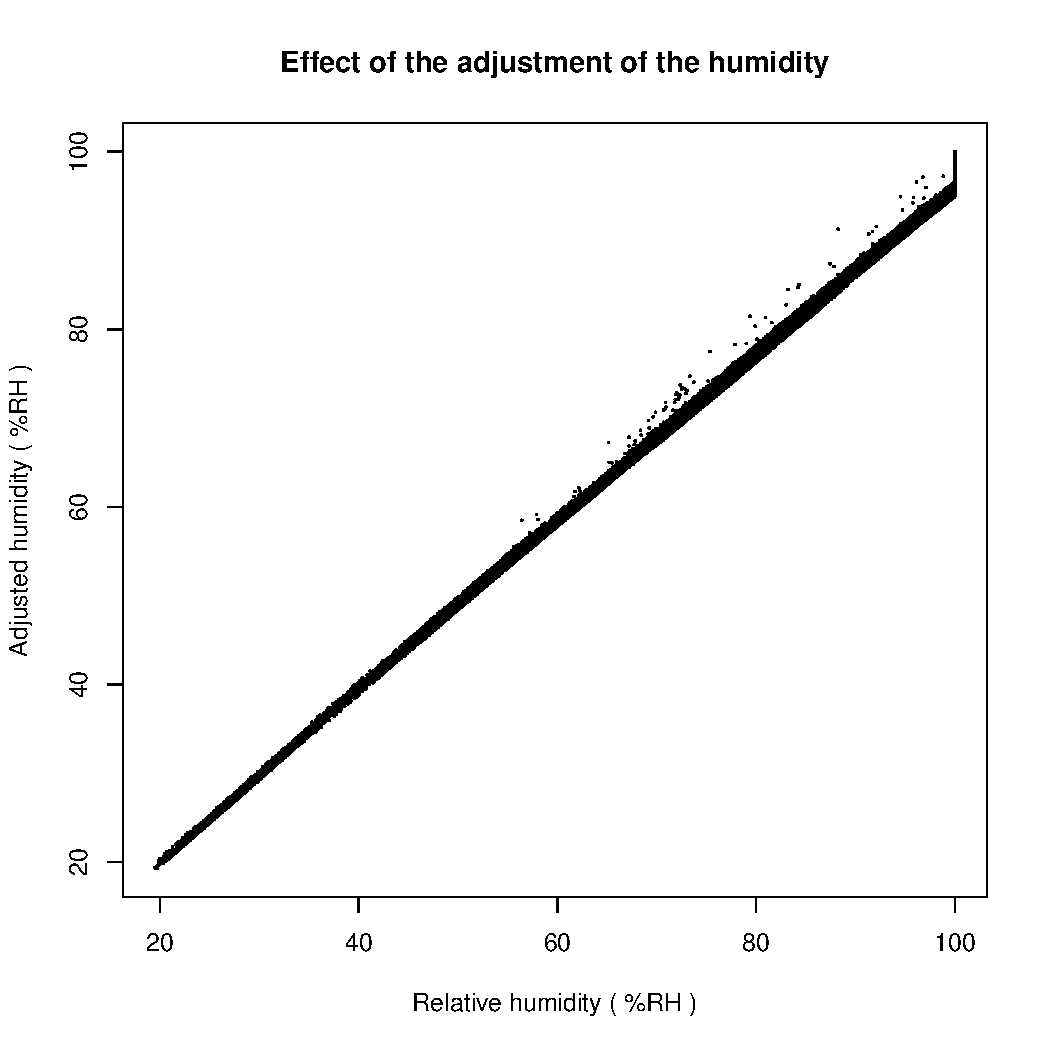
\includegraphics[width=0.6\linewidth]{figure/unnamed-chunk-7-1} 

}



\end{knitrout}


The third thing I want to check is the effect of the orientation of the sensors. It seems to me that since the Incident PAR sensor is measured on the top of the device, its value can be altered by the orientation of the device. To observe this phenomenon I propose to plot the distributions of the Incident PAR for each orientation and for each tranche of the day defined before. Here we do not have enough data for each of the orientations specified in the data set, so I will focus on the four of them for which I have most data: East South East (ESE), South (S), South East (SW) and West South West (WSW).


\section{Graphical Critique}
This is a critique of the plots in Figures 3 and 4 of the original paper \cite{tolle2005macroscope}. In  ~\ref{tab:obs}, we see the variables the study takes into account. However, the heights for figure 4 are not explicitly labeled as many lines are drawn for the two first plots. The authors could have added a gradient color in order to highlight some pattern in the humidity and temperature, should it exists any pattern. 
\begin{center}
   \begin{tabular}{| c | c | c | c | c | c | c |}
     \hline
     Variables & Time         & Temp         & RH          & Incident PAR & Reflected PAR& Height\\ \hline
     Figure 3a &              & $\checkmark$ &$\checkmark$ & $\checkmark$ & $\checkmark$ &             \\ \hline
     Figure 3b & $\checkmark$ & $\checkmark$ &$\checkmark$ & $\checkmark$ & $\checkmark$ &             \\ \hline
     Figure 3c &              & $\checkmark$ &$\checkmark$ & $\checkmark$ & $\checkmark$ & $\checkmark$\\ \hline
     Figure 3d &              & $\checkmark$ &$\checkmark$ & $\checkmark$ & $\checkmark$ & $\checkmark$\\ \hline
     Figure 4a & $\checkmark$ & $\checkmark$ &             &              &              & $\checkmark$\\ \hline
     Figure 4b & $\checkmark$ &              &$\checkmark$ &              &              & $\checkmark$\\ \hline
     Figure 4c & $\checkmark$ &              &             & $\checkmark$ &              & $\checkmark$\\ \hline
     Figure 4d & $\checkmark$ &              &             &              & $\checkmark$ & $\checkmark$\\
     \hline
   \end{tabular}
   \captionof{table}{Observations and variables of the figures 3 and 4 of the original data \cite{tolle2005macroscope}} \label{tab:obs} 
\end{center}
The authors try to identify patterns by projecting the three dimensional data (time, height and value) into two dimensional plots. Some of the conclusion drawn by the plots are, citing \cite{tolle2005macroscope}:
\begin{itemize}
\item All the nodes receive full sun occasionally
\item The reflected PAR sensors at the lower levels of the tree receive less light than higher sensors
\item Every sensor reached practically every point in the space of possible temperature and humidity readings
\item The lowest sensors in the tree are colder than average
\item Incident PAR follows the normal movement of the sun as it rises and then sets
\item Reflected PAR is more noisy
\item The temperature and the spread of temperatures throughout the tree increase as the sun rises
\item Temperature peaks in the afternoon, and then descends after the sun has set
\item Prior to sunrise, the humidity around the tree changes very quickly
\item  In the afternoon,humidity decreases overall, and after the sun sets, the spread in humidity reaches its lowest point
\end{itemize}
In my opinion, the boxplots in figure 3 of the original paper are hard to read, because there is too many boxplots for the area. I would rather gather some days, say sample every three days instead of every day. Moreover I think thet 3c and 3d are redundant and there is no need to put them together. As for figure 4, the data has been gathered one day, it would be better to have several other days to have an idea of the variance for example. Plus, the data used for the bottom left plot needs to be jittered in order to avoid the stratification. Finally the x axis of the bottom right plot of figure 4 needs to be adjusted.

\section{Findings}


\subsection{First finding}

In the right plot of Figure~\ref{fig:find1}, we observe that when the sun raises, around 7-8pm, the sensors on top of the tree record a higher level of PAR than the sensors on the bottom of the trees. This makes sense because at this time, the air is still cold but the effect of the sun make the top sensors warmer. Then, the temperature adjusts in the afternoon to finally decrease as the night goes on. We globally see that the top of the tree is warmer than the bottom. However, the perceived temperature might be higher when approaching the ground since the lowest part of the tree is sheltered from the wind.

The plot on the left highlights the fact that the top of the tree is significantly warmer than the bottom excepted in between noon and 4pm. What is not intuitive here is that the air on the top of the tree is warmer than the bottom at night. We can still notice that in the absence of wind, the heat would come up from the ground and heat the leaves.
\begin{figure}
  \centering
    \includegraphics[width=0.8\textwidth]{Find1.pdf}
  \caption{Difference of temperature between the top and the bottom of a tree of the Redwoods, for a typical day in the early summer. The left plot reports the distribution of the temperature of the sensors placed above 60 meters of the ground and the ones placed below 40 meters of the ground. The plot on the right highlights the same difference on an hour basis.}
  \label{fig:find1}
\end{figure}

\subsection{Second finding}

In Figure~\ref{fig:find2}, we notice that at a constant humidity rate, the temperatures are higher around noon. We also notice a linear relationship between the two variables: as humidity increases, the temperature decreases. This makes sense because when the nights come, the temperature decreases and the humidity increases and the inverse phenomenon is observed as the sun raises. 
\begin{figure}
  \centering
    \includegraphics[width=0.8\textwidth]{Find2}
  \caption{Distribution of the relative humidity and the temperature for different hours of the day. A gradient of colour is used to represent the different hours of the day: the orange points are the measures for data at 12pm and the blue points represent the measures at night.}
  \label{fig:find2}
\end{figure}


\subsection{Third finding}

In Figure~\ref{fig:find3}, we first notice that at night the incident PAR values are mostly near zero, which is expected since the sensors receive no sunlight. During the day however, we observe a concentration both near zero and near the top values. I infer that the low values correspond to the Incident PAR received by the captors near the ground and that the high values correspond to the sensors on the top of the tree. 

For each tranche of time, we observe that the orientation has little effect on the distribution of the incident PAR. However, the shape of the distribution of high values of PAR changes according to the orientation of the sensor. Indeed, we see a similar pattern for the SW orientation, which is different from the distribution of the PAR for the WSW orientation, no matter the tranche of the day we are looking at. We can say the same for the ESE orientation which leads to a different shape again.
\begin{figure}
  \centering
    \includegraphics[width=0.8\textwidth]{Find3}
  \caption{Effect of the orientation of the sensors placed on the trees over the distribution of the Incident PAR during  different periods of the day. A logarithmic scale is used for the PAR values.}
  \label{fig:find3}
\end{figure}


\section{Discussion}
For future work, one can study the stationarity hypothesis in order to see to which extent a typical day can be drawn. Moreover, one can highlights on Figure~\ref{fig:find2} the process of one day by drawing arrows and putting labels on points of the same day.

The variance of Figure~\ref{fig:find1} seems to be a bit too large to draw any conclusion, it might be better then to draw many of these plots for data gathered in periods of a week for example. It might also be wise to put an estimation of the temperature and humidity in the area and identify the differences with the ones in the trees. 

Finally, one can more precisely measure the effect of the orientation of the sensors on the measurements of Incident PCA by putting 4 sensors next to each other in the 4 cardinal directions. Then, we could possibly state whether the impact of the orientation of the sensors is significant or not.

\section{Conclusion}
The sensor network macroscope permits to validate some intuitive facts about the temperature, the humidity and the Incident PAR at different heights of the tree. This study shows that the use of the sensor network macroscope is promising in the sense that it is precise enough to have a consistent data set by removing obvious outliers and draw effective conclusions.

% the `Acknowledgments` section is required if you discussed the project
% with anyone else.
%\section*{Acknowledgments}


\bibliographystyle{plain}
\bibliography{bibli}

\end{document}
